\documentclass[11pt,a4paper]{article}

\usepackage[margin=2.5cm]{geometry}
\usepackage[T1]{fontenc}
\usepackage[utf8]{inputenc}
\usepackage{lmodern}
\usepackage{amsmath,amssymb}
\usepackage{booktabs}
\usepackage{array}
\usepackage{tabularx}
\usepackage{longtable}
\usepackage{graphicx}
\usepackage{xcolor}
\usepackage{float}
\usepackage{enumitem}
\usepackage{url}
\usepackage{hyperref}
\usepackage{caption}
\usepackage{subcaption}
\usepackage{microtype}

\graphicspath{{figures/}}
\hypersetup{
  colorlinks=true,
  linkcolor=blue,
  citecolor=blue,
  urlcolor=blue,
  pdfauthor={24376333 Huang Yibo; 24376267 Wang Xihao; 24301017 Yang Xiaochu},
  pdftitle={KITTI Visual SLAM Baseline Comparative Report}
}
\urlstyle{same}

\newcolumntype{Y}{>{\raggedright\arraybackslash}X}
\newcommand{\NA}{\textsc{N/A}}
\newcommand{\paperclaim}{\texttt{paper\_level\_claim=false}}
\newcommand{\methodorb}{ORB-SLAM2-inspired stereo SLAM}
\newcommand{\methoddso}{DSO-inspired direct sparse stereo SLAM}
\newcommand{\methodsvo}{SVO-style semi-direct stereo visual odometry/SLAM}

\title{A Comparative Study of ORB-Style, DSO-Style, and SVO-Style Visual SLAM Baselines on KITTI}
\author{\large\bfseries 24376333 Huang Yibo \quad 24376267 Wang Xihao \quad 24301017 Yang Xiaochu\\[0.3em]
Machine Learning Course Project}
\date{\today}

\begin{document}
\maketitle

\section{Title}

The title of this report is \emph{A Comparative Study of ORB-Style, DSO-Style, and SVO-Style Visual SLAM Baselines on KITTI}. The report studies three Python research baselines: \methodorb{}, \methoddso{}, and \methodsvo{}. The central objective is to compare feature-based, direct sparse, and semi-direct visual SLAM/VO designs under a unified KITTI Odometry benchmark. The report focuses on implementation-level behavior, experimental reproducibility, and diagnostic analysis rather than claiming full reproduction of the original official systems.

\section{Background and Significance}

Simultaneous localization and mapping (SLAM) is a fundamental problem in mobile robotics and autonomous driving. Its objective is to estimate the motion trajectory of a sensor platform while maintaining a representation of the surrounding environment. Visual SLAM is especially important because cameras are inexpensive, compact, and information-rich sensors. A stereo camera sequence can provide both texture and metric depth cues, making it suitable for vehicle-scale trajectory estimation. At the same time, visual SLAM is sensitive to illumination variation, motion blur, low texture, repeated patterns, calibration quality, and data-association errors.

Classical visual SLAM and visual odometry (VO) systems can be broadly grouped into three design families. Feature-based systems represent images using repeatable keypoints and descriptors, and then estimate motion using geometric constraints. Direct sparse systems optimize photometric residuals over selected pixels and can avoid explicit descriptor matching, but they require careful photometric modeling and reliable initialization. Semi-direct systems combine sparse map structure with patch-level or optical-flow tracking, aiming to achieve a compromise between geometric robustness and computational efficiency.

The significance of this project is that it implements and evaluates these three families in one consistent Python framework. The implementation is not intended to match production-grade C++ systems. Instead, it provides reproducible research baselines that share the same KITTI stereo input, calibration interface, trajectory output format, evaluation script, JSON reporting schema, and alignment setting. This design makes the comparison controlled enough to reveal implementation-level differences while avoiding overclaims about the full ORB-SLAM2, DSO, or SVO systems.

The report addresses three research questions:
\begin{enumerate}[leftmargin=2em]
  \item Under the same KITTI sequence, frame count, alignment setting, and evaluation code, how do the three Python baselines differ in trajectory accuracy and robustness?
  \item Does the SVO-style semi-direct baseline provide an observable trade-off between the stability of the ORB-style baseline and the speed of lighter-weight tracking?
  \item Which implementation factors explain the drift and failures observed in the DSO-style baseline, and do grid-uniform point selection and outlier culling reduce catastrophic drift?
\end{enumerate}

The project manifest keeps \paperclaim{}. This statement is important: the repository provides reproducible Python baselines inspired by classical SLAM systems, not official full paper-level reproductions.

\section{Literature Review}

\subsection{Feature-Based Visual SLAM}

Feature-based visual SLAM converts images into sparse keypoints and descriptors. Camera motion and map structure are then estimated using feature matching, geometric verification, triangulation, PnP, and bundle adjustment. ORB-SLAM2 is a representative feature-based system for monocular, stereo, and RGB-D cameras. It combines ORB features, keyframe-based mapping, local bundle adjustment, relocalization, and loop closing \cite{mur2017orbslam2}. The ORB descriptor itself was introduced as an efficient alternative to SIFT and SURF and is widely used in real-time visual systems \cite{rublee2011orb}.

The strength of feature-based SLAM is that its correspondences have explicit geometric meaning, and robust methods such as RANSAC can reject many outliers before pose estimation. This makes feature-based pipelines relatively stable when repeatable texture is available. Their limitations include the computational cost of descriptor extraction and matching, sensitivity to low-texture scenes, and the engineering complexity of mature map management. The ORB-style baseline in this project implements the main stereo feature-based ideas, including stereo depth, ORB features, 3D-2D PnP RANSAC, keyframes, and local map structures. It does not claim to reproduce the full maturity of official ORB-SLAM2.

\subsection{Direct Sparse Odometry}

Direct methods avoid explicit descriptor matching and estimate motion by minimizing intensity or photometric residuals. Direct Sparse Odometry (DSO) selects high-gradient pixels and jointly optimizes camera poses, inverse depths, and photometric parameters in a sparse direct formulation \cite{engel2018dso}. Full DSO relies on calibrated photometric response handling, sparse direct bundle adjustment, active-window marginalization, and carefully managed point lifecycles.

The potential advantage of direct sparse methods is that they can use image information that is not captured by sparse descriptors. However, they are also sensitive to the validity of the brightness constancy assumption, exposure changes, initialization errors, and nonconvex optimization. The DSO-style implementation in this project is a simplified Python baseline. It includes stereo initialization, high-gradient sparse points, an inverse-depth active window, LK+PnP initialization, simplified photometric refinement, motion gating, fallback, and diagnostics. It does not implement complete Schur-complement marginalization, full photometric bundle adjustment, calibrated exposure/response/vignetting modeling, or production-level point lifecycle management. Therefore, drift observed in this baseline should be interpreted as an implementation-level limitation rather than a failure of the original DSO method.

\subsection{Semi-Direct Visual Odometry}

SVO introduced a semi-direct visual odometry approach that combines sparse map structure with direct image alignment \cite{forster2014svo}. The key idea is to avoid expensive descriptor matching during frame-to-frame tracking while still maintaining sparse geometric constraints. Semi-direct methods commonly use patch alignment or optical flow to track projected map points, and then use geometric pose estimation to obtain camera motion.

The SVO-style baseline in this project follows this design philosophy. It uses grid-uniform sparse point selection, stereo depth initialization, pyramidal Lucas-Kanade optical flow for patch-level tracking, 3D-2D PnP RANSAC for pose estimation, and keyframe refresh for local map maintenance. Lucas-Kanade tracking provides the basis for iterative patch alignment \cite{lucas1981iterative}, while RANSAC provides robust geometric model selection \cite{fischler1981random}. This baseline does not include the full SVO probabilistic depth filter, mature backend, production relocalization, or loop closure.

\subsection{KITTI and Modern Deep SLAM}

The KITTI Vision Benchmark Suite provides outdoor driving datasets and benchmark tasks for stereo vision, optical flow, visual odometry, SLAM, and related autonomous-driving problems \cite{geiger2012kitti}. This project uses KITTI Odometry sequence 00 because it provides stereo images and a ground-truth trajectory suitable for controlled VO/SLAM comparison.

Recent deep learning systems such as DROID-SLAM and DPVO achieve strong performance by combining neural matching or update models with differentiable optimization \cite{teed2021droidslam,teed2023dpvo}. These systems are important related work, but they require pretrained models, GPU-oriented inference, and a different engineering stack. For an implementation-oriented course project focused on classical SLAM baselines, they are discussed as related work rather than included as primary algorithms.

\section{Methodological Principles}

\subsection{Unified Benchmark Framework}

All three methods use the same KITTI stereo loader, calibration data, trajectory format, evaluation script, and JSON reporting logic. Each input frame must produce one $4\times4$ pose matrix. When tracking fails, the system must keep the trajectory length unchanged by using fallback or the previous safe pose. Failed frames are not removed, and trajectories are not silently truncated. This rule is essential because otherwise the evaluation could become artificially favorable to unstable methods.

Figure~\ref{fig:workflow} shows the shared benchmark workflow. The ORB-style frontend uses feature matching and geometric estimation. The DSO-style frontend uses sparse photometric residuals after LK+PnP initialization. The SVO-style frontend uses patch or optical-flow tracking followed by PnP. The three methods then share the same output layer: trajectory files, benchmark JSON, trajectory plots, and diagnostics plots.

\begin{figure}[H]
  \centering
  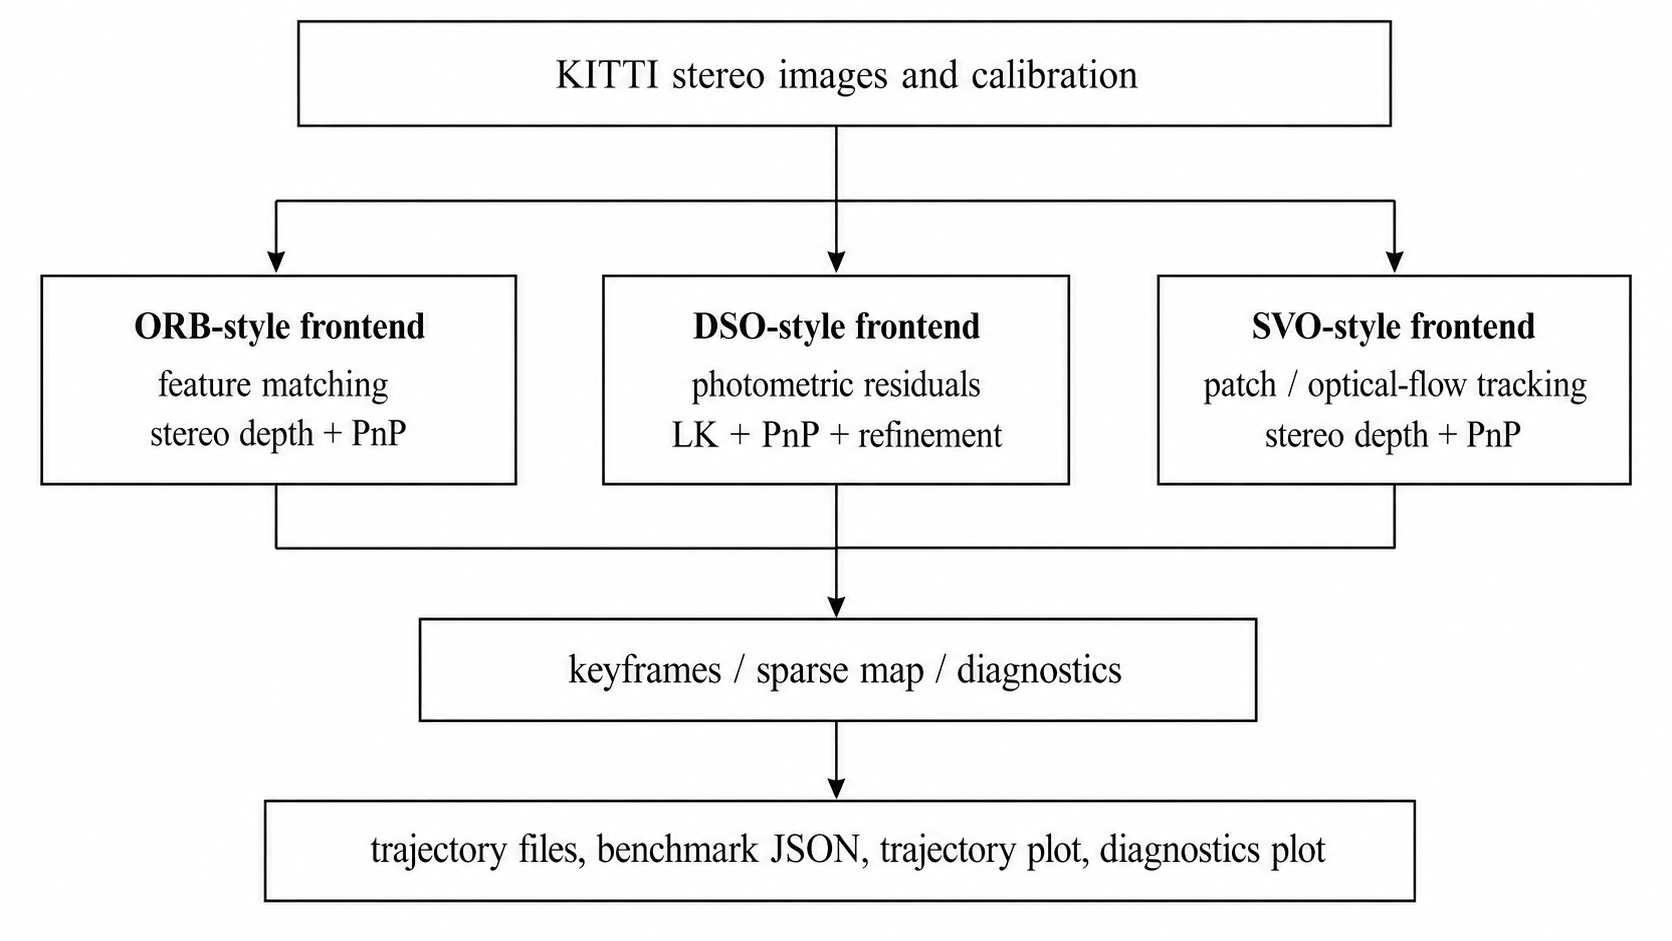
\includegraphics[width=0.92\textwidth]{Workflow.png}
  \caption{Shared benchmark workflow for the three Python SLAM/VO baselines. The figure is loaded from \texttt{figures/Workflow.png}.}
  \label{fig:workflow}
\end{figure}

\subsection{ORB-SLAM2-Inspired Stereo SLAM}

The ORB-style baseline detects ORB features in stereo images and initializes sparse 3D points from stereo disparity. Pose estimation uses correspondences between local 3D map points and current-frame 2D features. PnP with RANSAC is used to estimate camera motion and reject inconsistent matches. New keyframes are inserted when tracking quality, parallax, or motion thresholds indicate that the current local map should be refreshed.

The geometric pose estimation problem can be written as robust reprojection-error minimization:
\begin{equation}
  \min_{T\in SE(3)} \sum_{i\in\mathcal{I}} \rho\left(\left\|u_i - \pi(TP_i)\right\|_2^2\right),
\end{equation}
where $P_i$ is a 3D map point, $u_i$ is its current 2D observation, $\pi(\cdot)$ is the calibrated camera projection function, $T$ is the current pose, and $\rho$ denotes a robust loss or the inlier set selected by RANSAC. The baseline contains keyframes, map points, local map tracking, and loop-count statistics. In the reported experiments, the number of loop closures is zero.

\subsection{DSO-Inspired Direct Sparse Stereo SLAM}

The DSO-style baseline selects sparse high-gradient locations with valid stereo depth. Given a reference image $I_r$ and a current image $I_t$, the photometric residual for a sparse 3D point $P_i$ can be expressed as
\begin{equation}
  r_i(\xi)=I_t\left(\pi(\exp(\xi)P_i)\right)-I_r(u_i),
\end{equation}
where $\xi$ is a pose increment in the Lie algebra of $SE(3)$. The simplified photometric objective is
\begin{equation}
  E_{\mathrm{photo}}(\xi)=\sum_{i\in\Omega}\rho\left(r_i(\xi)^2\right),
\end{equation}
where $\Omega$ is the set of sparse points that can be validly projected into the current image.

To reduce implementation-level drift, the final main experiment enables grid-uniform high-gradient point selection, depth range filtering, photometric residual outlier culling, low valid-projection rejection, motion gating, and fallback. The motion gate checks whether the estimated frame-to-frame translation or rotation is implausible. When the photometric refinement candidate is rejected, the system falls back to LK+PnP, constant velocity, or the previous safe pose. Per-frame diagnostics record tracking cost, valid projected points, residual mean, residual median, residual 95th percentile, inlier ratio, relative motion, failure flag, fallback flag, keyframe insertion, and active inverse-depth points.

\subsection{SVO-Style Semi-Direct Stereo VO/SLAM}

The SVO-style baseline lies between the feature-based and direct sparse pipelines. It does not rely on ORB descriptor matching as its primary tracking mechanism. Instead, sparse points from the reference keyframe are tracked in the current frame using pyramidal Lucas-Kanade optical flow or patch-level alignment. The tracked 2D locations are paired with reference-frame 3D points, and solvePnPRansac estimates the current pose from these 3D-2D correspondences.

This design preserves stereo depth initialization and sparse geometric verification while avoiding the cost of full descriptor matching in every frame. Keyframe insertion is triggered by tracked point count, PnP inlier ratio, parallax, translation, rotation, or the elapsed number of frames since the last keyframe. The reported SVO-style baseline records keyframes, active sparse points, tracking failures, fallback count, loop-closure status, mean tracked points, and mean PnP inliers. Production-grade loop closure is not enabled, and loop closures are reported as zero.

\subsection{Evaluation Metrics and Fairness Controls}

The main accuracy metric is origin-aligned absolute trajectory error (ATE) RMSE:
\begin{equation}
  \mathrm{ATE}_{\mathrm{RMSE}} = \sqrt{\frac{1}{N}\sum_{i=1}^{N}\left\|\mathrm{trans}\left((T_i^{\mathrm{gt}})^{-1}AT_i^{\mathrm{est}}\right)\right\|_2^2},
\end{equation}
where $T_i^{\mathrm{gt}}$ is the ground-truth pose, $T_i^{\mathrm{est}}$ is the estimated pose, and $A$ is the alignment transform. The benchmark also stores relative pose error (RPE), KITTI-style segment metrics, runtime average/median/95th percentile, wall time, keyframe count, tracking failures, fallbacks, loop closures, and method-specific robustness statistics.

Fairness controls include the same KITTI sequence, the same frame count, the same origin alignment, the same trajectory output format, the same evaluation code, and strict trajectory-length checking. All JSON outputs are standard JSON files; non-finite values such as NaN and infinity are converted to \texttt{null}. In the final 100-frame run, RPE and KITTI segment metrics are \texttt{null} because the short subsequence does not provide the 100 m to 800 m path segments required by the metric implementation. These fields are therefore reported as \NA{} rather than imputed.

\section{Experimental Results and Analysis}

\subsection{Experimental Setup}

The final main experiment uses the first 100 frames of KITTI Odometry sequence 00. The selected output directory is
\begin{center}
\texttt{results/final\_seq00\_100\_stabilized\_f800\_p800}.
\end{center}
The configuration is: ORB features = 800, DSO points = 800, SVO points = 800, and alignment = origin. The DSO main configuration enables grid selection, outlier culling, motion gate, and photometric refinement. Its fallback mode is LK+PnP, then constant velocity, then the previous safe pose.

A previous 100-frame run using 1500 ORB features was excluded from final runtime analysis because its wall-time measurement was contaminated by a local power interruption or sleep event. A 300-frame run was not included in the final report because the Python ORB-style baseline was computationally expensive under high feature settings. Since hardware specifications were not separately logged, runtime values should be treated as within-run comparisons on the same local workstation rather than portable hardware-normalized claims.

Table~\ref{tab:components} summarizes the implemented components and omitted full-system components. This distinction is necessary because the three baselines differ in backend maturity. The comparison is therefore a project-level baseline comparison, not a claim about the maximum performance of the official systems.

\begin{table}[H]
\centering
\scriptsize
\caption{Implemented components and known omissions of the three visual SLAM/VO baselines.}
\label{tab:components}
\begin{tabularx}{\textwidth}{p{0.16\textwidth}YYY}
\toprule
Category & ORB-SLAM2-inspired stereo SLAM & DSO-inspired direct sparse stereo SLAM & SVO-style semi-direct stereo VO/SLAM \\
\midrule
Frontend & ORB feature extraction, sparse matching, and geometric verification & High-gradient sparse points, photometric residuals, and LK+PnP initialization & Grid-uniform sparse points with patch/optical-flow tracking \\
Depth initialization & Stereo disparity and metric depth & Stereo depth and inverse-depth active points & Stereo depth initialization for reference sparse points \\
Pose estimation & 3D-2D PnP RANSAC and local tracking & LK+PnP plus simplified photometric refinement & Optical-flow tracks plus 3D-2D PnP RANSAC \\
Keyframes and map & Keyframes, map points, and local mapping structures & Active keyframe window and inverse-depth points & Keyframes, active sparse points, and local map refresh \\
Robustness & Tracking-failure statistics; loop closures are zero in the reported run & Motion gate, outlier culling, fallback, and per-frame diagnostics & Motion gate, PnP inlier filtering, and fallback \\
Missing full-system components & Full official ORB-SLAM2 maturity, large-scale vocabulary behavior, and complete production backend & Full photometric BA, exposure/response/vignetting calibration, Schur-complement marginalization, and mature point lifecycle & Full SVO probabilistic depth filter, mature backend, production relocalization, and loop closure \\
\bottomrule
\end{tabularx}
\end{table}

\subsection{Main 100-Frame Results}

Table~\ref{tab:main-results} reports the final 100-frame comparison. The ORB-style baseline obtains the lowest ATE RMSE, 1.8984 m, with zero tracking failures. The SVO-style baseline obtains 2.3916 m ATE RMSE with zero tracking failures and a much lower wall time of 8.54 s. The DSO-style baseline obtains 9.4367 m ATE RMSE and records 9 tracking failures with 9 fallbacks, indicating that the simplified direct sparse implementation still suffers from implementation-level drift.

\begin{table}[H]
\centering
\small
\caption{Main 100-frame results on KITTI sequence 00. Configuration: origin alignment, 800 ORB features, 800 DSO points, and 800 SVO points. RPE and KITTI segment metrics are \NA{} because the corresponding benchmark JSON fields are \texttt{null}.}
\label{tab:main-results}
\resizebox{\textwidth}{!}{%
\begin{tabular}{lccccccccc}
\toprule
Algorithm & ATE RMSE (m) & RPE trans & RPE rot & Runtime avg/median/p95 (ms) & Wall time (s) & Keyframes & Failures & Fallbacks & Loop closures \\
\midrule
ORB & 1.8984 & \NA{} & \NA{} & 6827.45 / 66.42 / 30549.24 & 687.68 & 34 & 0 & \NA{} & 0 \\
DSO & 9.4367 & \NA{} & \NA{} & 779.06 / 418.88 / 2101.41 & 79.03 & 39 & 9 & 9 & 0 \\
SVO & 2.3916 & \NA{} & \NA{} & 73.34 / 89.86 / 101.11 & 8.54 & 75 & 0 & 0 & 0 \\
\bottomrule
\end{tabular}}
\end{table}

Figure~\ref{fig:final-traj} shows the trajectory comparison. The ORB-style and SVO-style trajectories remain closer to the ground-truth trajectory, while the DSO-style trajectory shows a visible deviation in the later part of the sequence. This is consistent with the higher DSO ATE and the recorded tracking failures.

\begin{figure}[H]
  \centering
  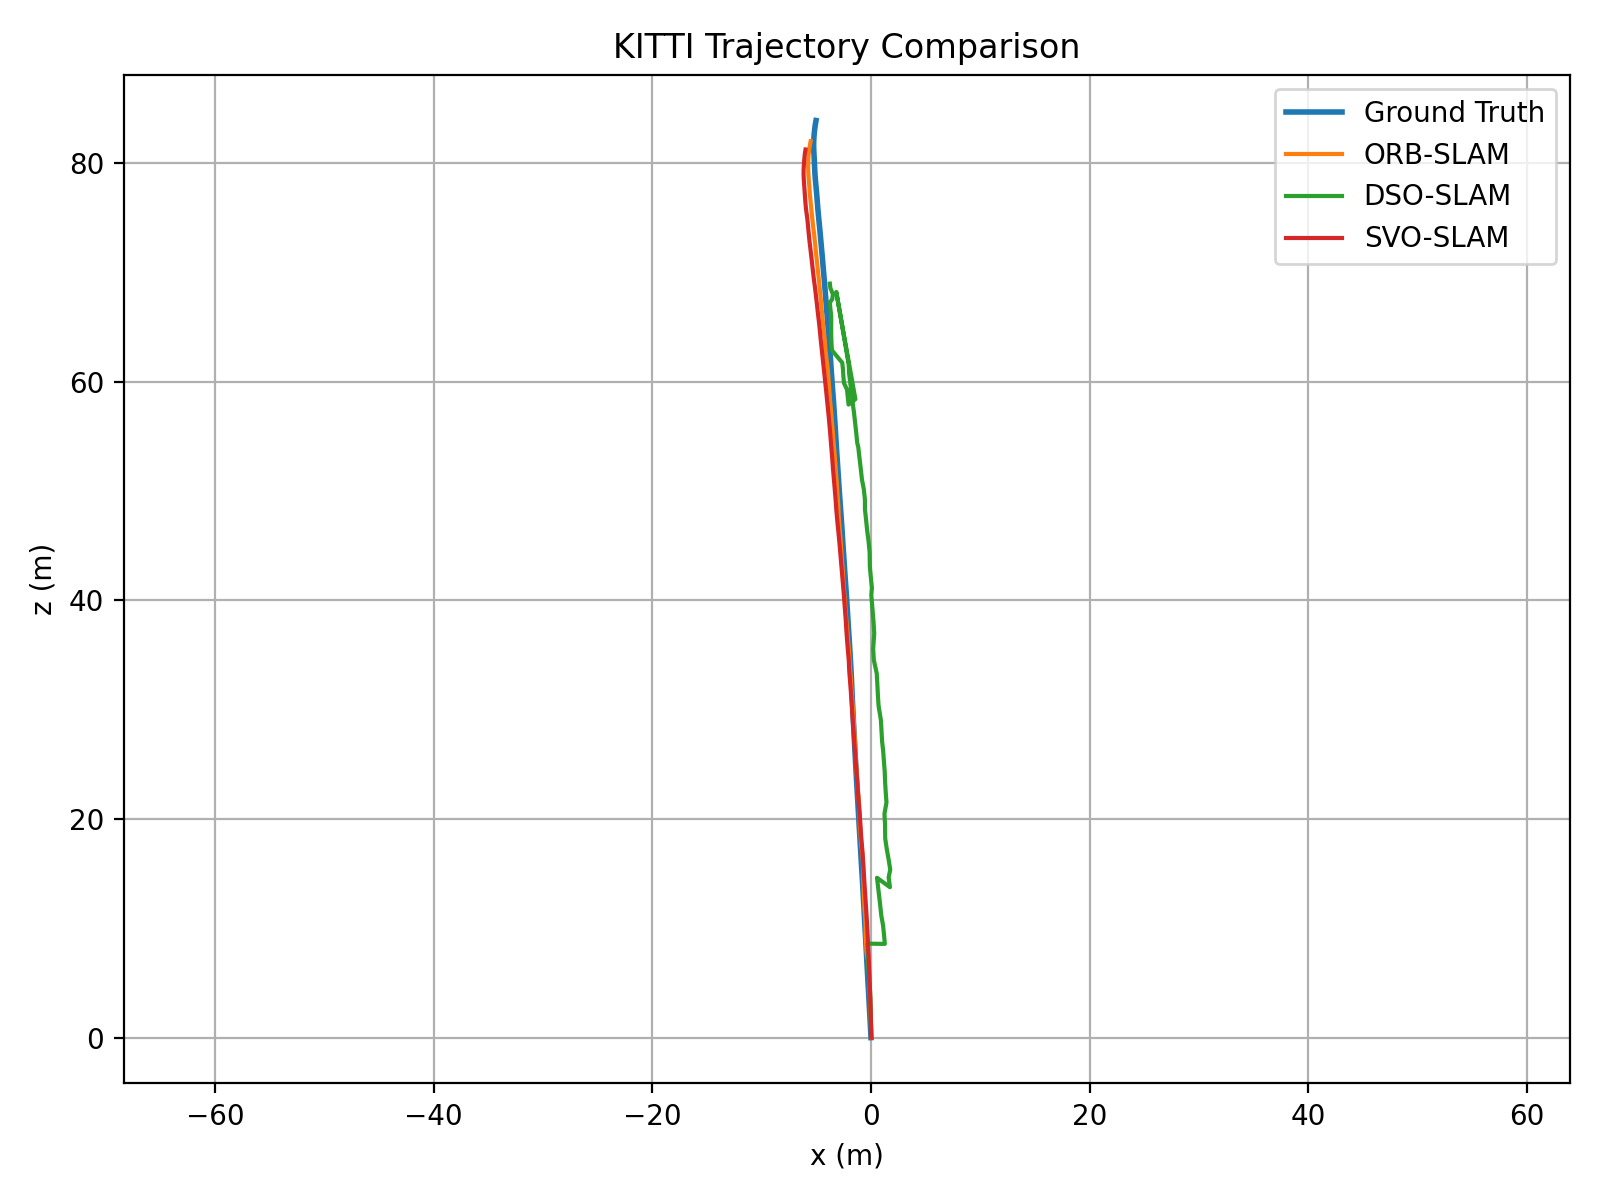
\includegraphics[width=0.76\textwidth]{final_trajectory_seq00.png}
  \caption{Trajectory comparison for the first 100 frames of KITTI sequence 00. The figure includes ground truth, ORB-style, DSO-style, and SVO-style trajectories.}
  \label{fig:final-traj}
\end{figure}

\subsection{Robustness and DSO Diagnostics}

Table~\ref{tab:diagnostics} summarizes robustness statistics for the final 100-frame run. The DSO-style baseline has a mean valid projected point count of 599.62 and a mean inlier ratio of 0.6995. However, diagnostics show a contiguous failure interval around frames 71--79. The maximum relative translation is 11.4520 m and the maximum relative rotation is 9.5412 degrees, indicating that some photometric refinement candidates still produce implausible frame-to-frame motion and require motion-gate rejection or fallback.

\begin{table}[H]
\centering
\small
\caption{Robustness and DSO diagnostics summary for the final 100-frame run. DSO residual statistics are from \texttt{dso\_diagnostics\_seq00.json}.}
\label{tab:diagnostics}
\begin{tabular}{lccc}
\toprule
Statistic & ORB & DSO & SVO \\
\midrule
Frames processed & 100 & 100 & 100 \\
Keyframes & 34 & 39 & 75 \\
Tracking failures & 0 & 9 & 0 \\
Fallbacks & \NA{} & 9 & 0 \\
Motion gate rejections & \NA{} & 8 & 0 \\
Loop closures & 0 & 0 & 0 \\
Mean valid projected/tracked points & \NA{} & 599.62 & 563.94 \\
Median valid projected/tracked points & \NA{} & 606.50 & 574.00 \\
Mean inlier ratio & \NA{} & 0.6995 & 0.7554 \\
Mean PnP inliers & \NA{} & \NA{} & 428.97 \\
Mean residual mean & \NA{} & 24.8132 & \NA{} \\
Median residual median & \NA{} & 10.8250 & \NA{} \\
Mean residual p95 & \NA{} & 85.9493 & \NA{} \\
Max relative translation (m) & \NA{} & 11.4520 & \NA{} \\
Max relative rotation (deg) & \NA{} & 9.5412 & \NA{} \\
Active sparse/inverse-depth points & \NA{} & 3000 & 3951 \\
\bottomrule
\end{tabular}
\end{table}

Figure~\ref{fig:dso-diag} visualizes DSO valid projected points, inlier ratio, and failure flags over time. The failure interval is associated with a decline in valid points and inlier quality. This supports the interpretation that DSO drift is caused not only by large candidate motion, but also by residual-set quality, spatial coverage, and initialization stability.

\begin{figure}[H]
  \centering
  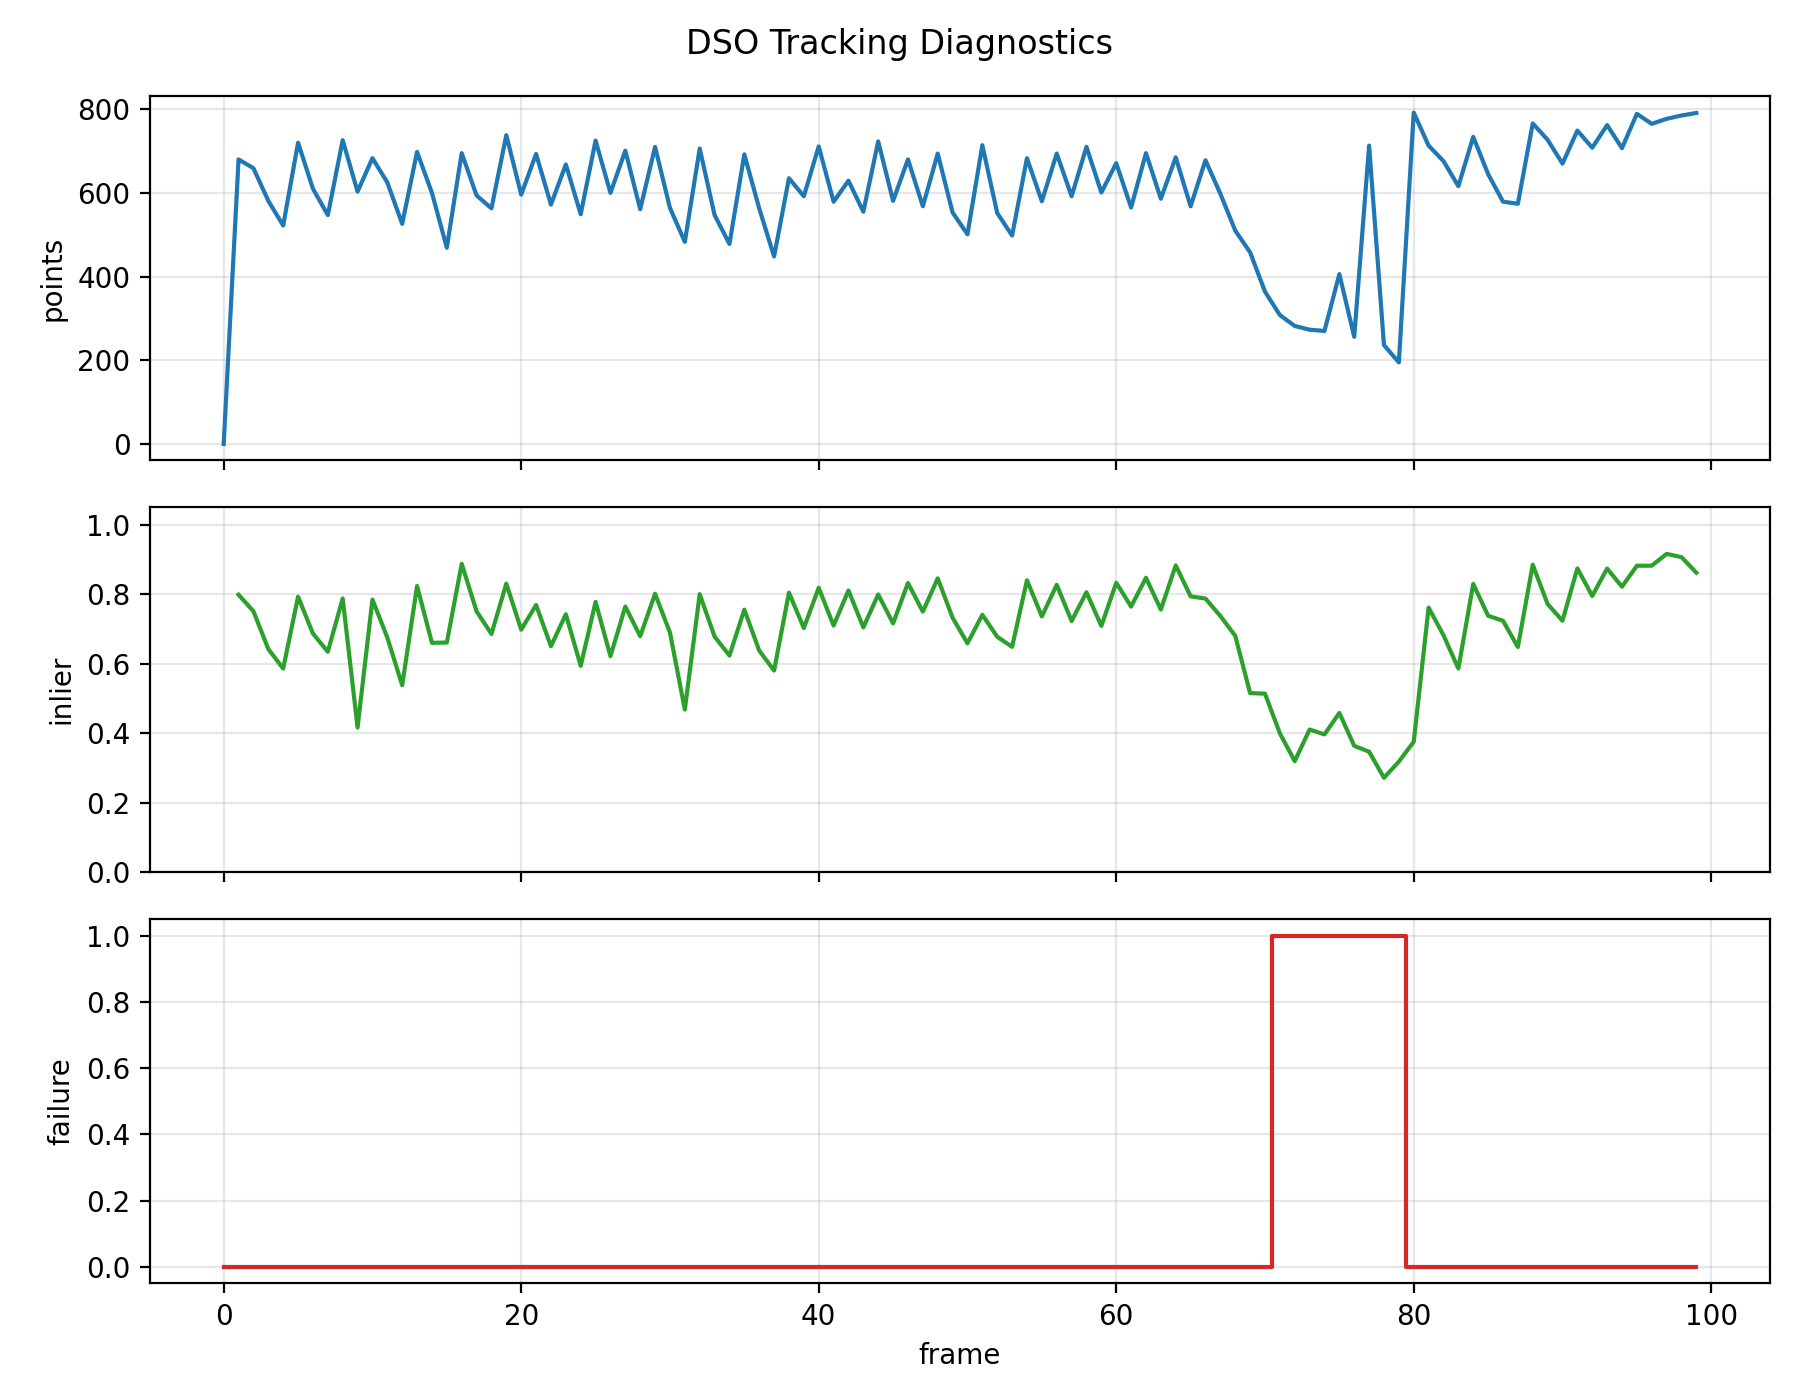
\includegraphics[width=0.76\textwidth]{final_dso_diagnostics_seq00.png}
  \caption{DSO diagnostics for the final 100-frame stabilized run. The plot shows valid projected points, inlier ratio, and the failure interval around frames 71--79.}
  \label{fig:dso-diag}
\end{figure}

\subsection{DSO Ablation Study}

To explain the drift of the DSO-style baseline more precisely, a 100-frame DSO ablation was run with 1500 sparse points. Table~\ref{tab:dso-ablation} shows that grid-uniform point selection reduces ATE RMSE to 11.6835 m, while the outlier-culling-on configuration reaches 9.5661 m. In contrast, the photometric-with-motion-gate and outlier-culling-off configurations remain around 75.8 m. This result shows that motion gating alone is insufficient when the photometric residual set contains many unstable points.

\begin{table}[H]
\centering
\scriptsize
\caption{DSO ablation on KITTI sequence 00, 100 frames, and 1500 sparse points. These results diagnose the simplified DSO-style baseline and are not claims about full DSO.}
\label{tab:dso-ablation}
\resizebox{\textwidth}{!}{%
\begin{tabular}{lrrrrrrr}
\toprule
Configuration & ATE RMSE (m) & Failures & Fallbacks & Motion gate & Mean valid pts & Mean inlier & Runtime avg (ms) \\
\midrule
full\_simplified\_dso & 40.0404 & 1 & 1 & 0 & 1113.22 & 0.7338 & 734.29 \\
lk\_pnp\_only & 77.2572 & 0 & 0 & 0 & 1115.00 & 0.6717 & 616.25 \\
photometric\_with\_motion\_gate & 75.7913 & 17 & 17 & 10 & 1346.86 & 0.4826 & 534.43 \\
grid\_uniform\_selection & 11.6835 & 1 & 1 & 0 & 1113.49 & 0.7381 & 836.57 \\
outlier\_culling\_on & 9.5661 & 14 & 14 & 10 & 1361.77 & 0.4819 & 593.63 \\
outlier\_culling\_off & 75.7913 & 17 & 17 & 10 & 1346.86 & 0.4826 & 535.78 \\
\bottomrule
\end{tabular}}
\end{table}

Figure~\ref{fig:dso-ablation} shows the ablation results. Although the outlier-culling-on configuration still has many fallbacks, its ATE is much lower than configurations without effective outlier control. Therefore, the number of fallbacks alone is not the main indicator of accuracy. The more important factor is whether unstable residuals are rejected before they corrupt accepted pose updates.

\begin{figure}[H]
  \centering
  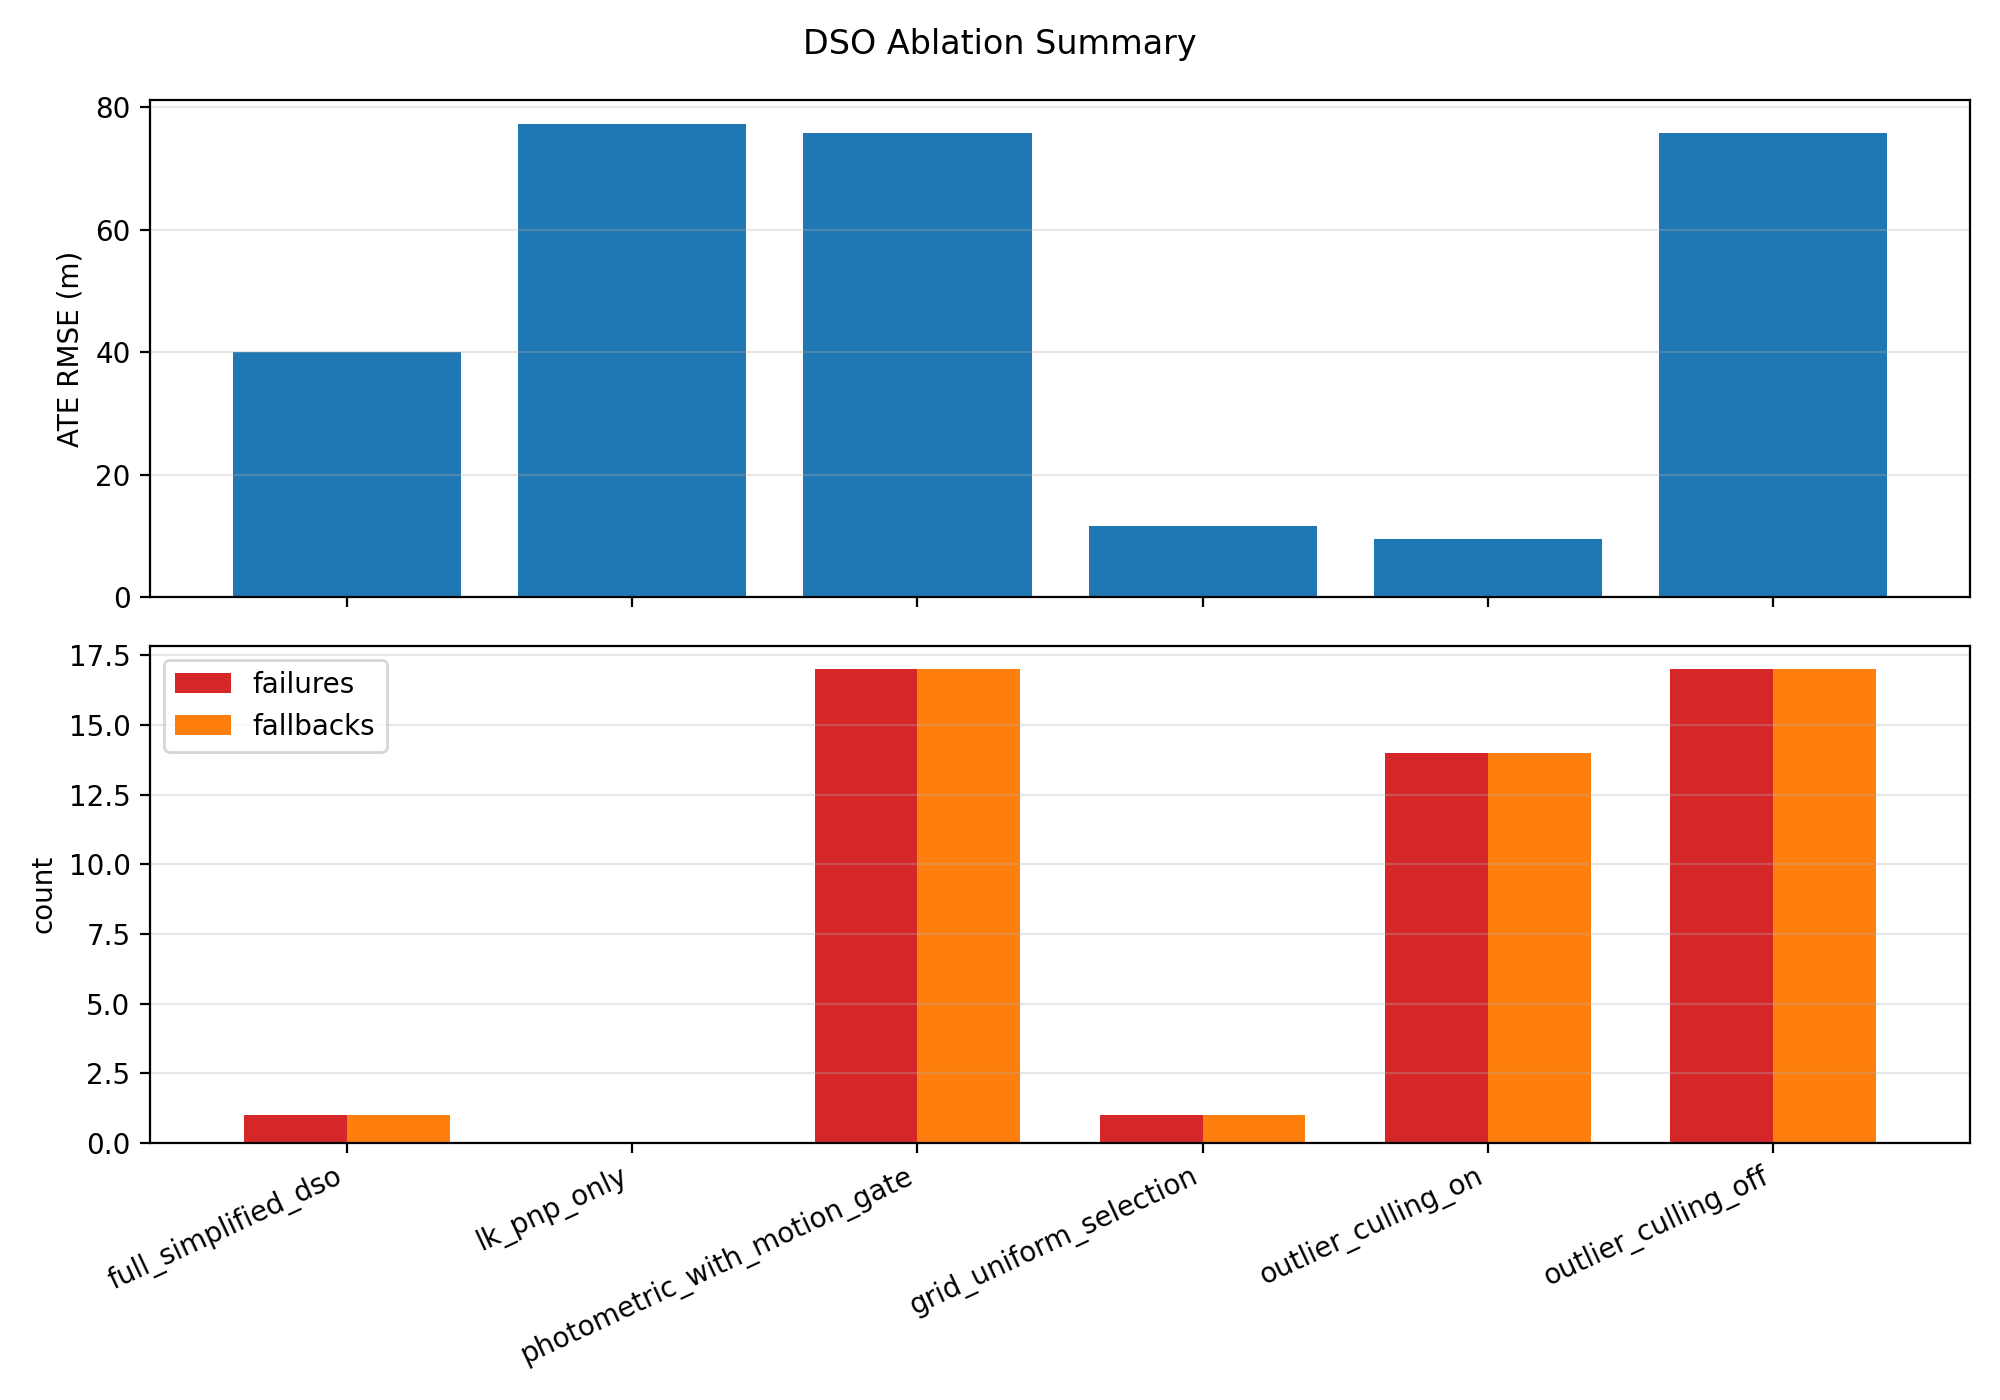
\includegraphics[width=0.76\textwidth]{dso_ablation_seq00.png}
  \caption{DSO ablation plot for the 100-frame, 1500-point experiment. The upper plot reports ATE RMSE, and the lower plot reports failures and fallbacks.}
  \label{fig:dso-ablation}
\end{figure}

\subsection{20-Frame Sanity Check}

The 20-frame experiment is used as a sanity check to verify that all three pipelines run end-to-end and output trajectories with aligned lengths. Table~\ref{tab:sanity} and Figure~\ref{fig:sanity-traj} show that all three methods finish the short run without tracking failures. The ORB-style ATE is 0.9367 m, the SVO-style ATE is 1.1066 m, and the DSO-style ATE is 1.6427 m. Because the sequence is very short, this run should not be overinterpreted as a final performance result; it mainly confirms benchmark integration and basic tracking functionality.

\begin{table}[H]
\centering
\small
\caption{20-frame sanity-check results on KITTI sequence 00.}
\label{tab:sanity}
\resizebox{\textwidth}{!}{%
\begin{tabular}{lrrrrrrr}
\toprule
Algorithm & ATE RMSE (m) & Runtime avg/median/p95 (ms) & Wall time (s) & Keyframes & Failures & Fallbacks & Loops \\
\midrule
ORB & 0.9367 & 6078.94 / 91.78 / 28712.37 & 121.92 & 7 & 0 & \NA{} & 0 \\
DSO & 1.6427 & 610.33 / 386.47 / 1216.79 & 12.16 & 7 & 0 & 0 & 0 \\
SVO & 1.1066 & 118.25 / 163.89 / 189.46 & 2.76 & 12 & 0 & 0 & 0 \\
\bottomrule
\end{tabular}}
\end{table}

\begin{figure}[H]
  \centering
  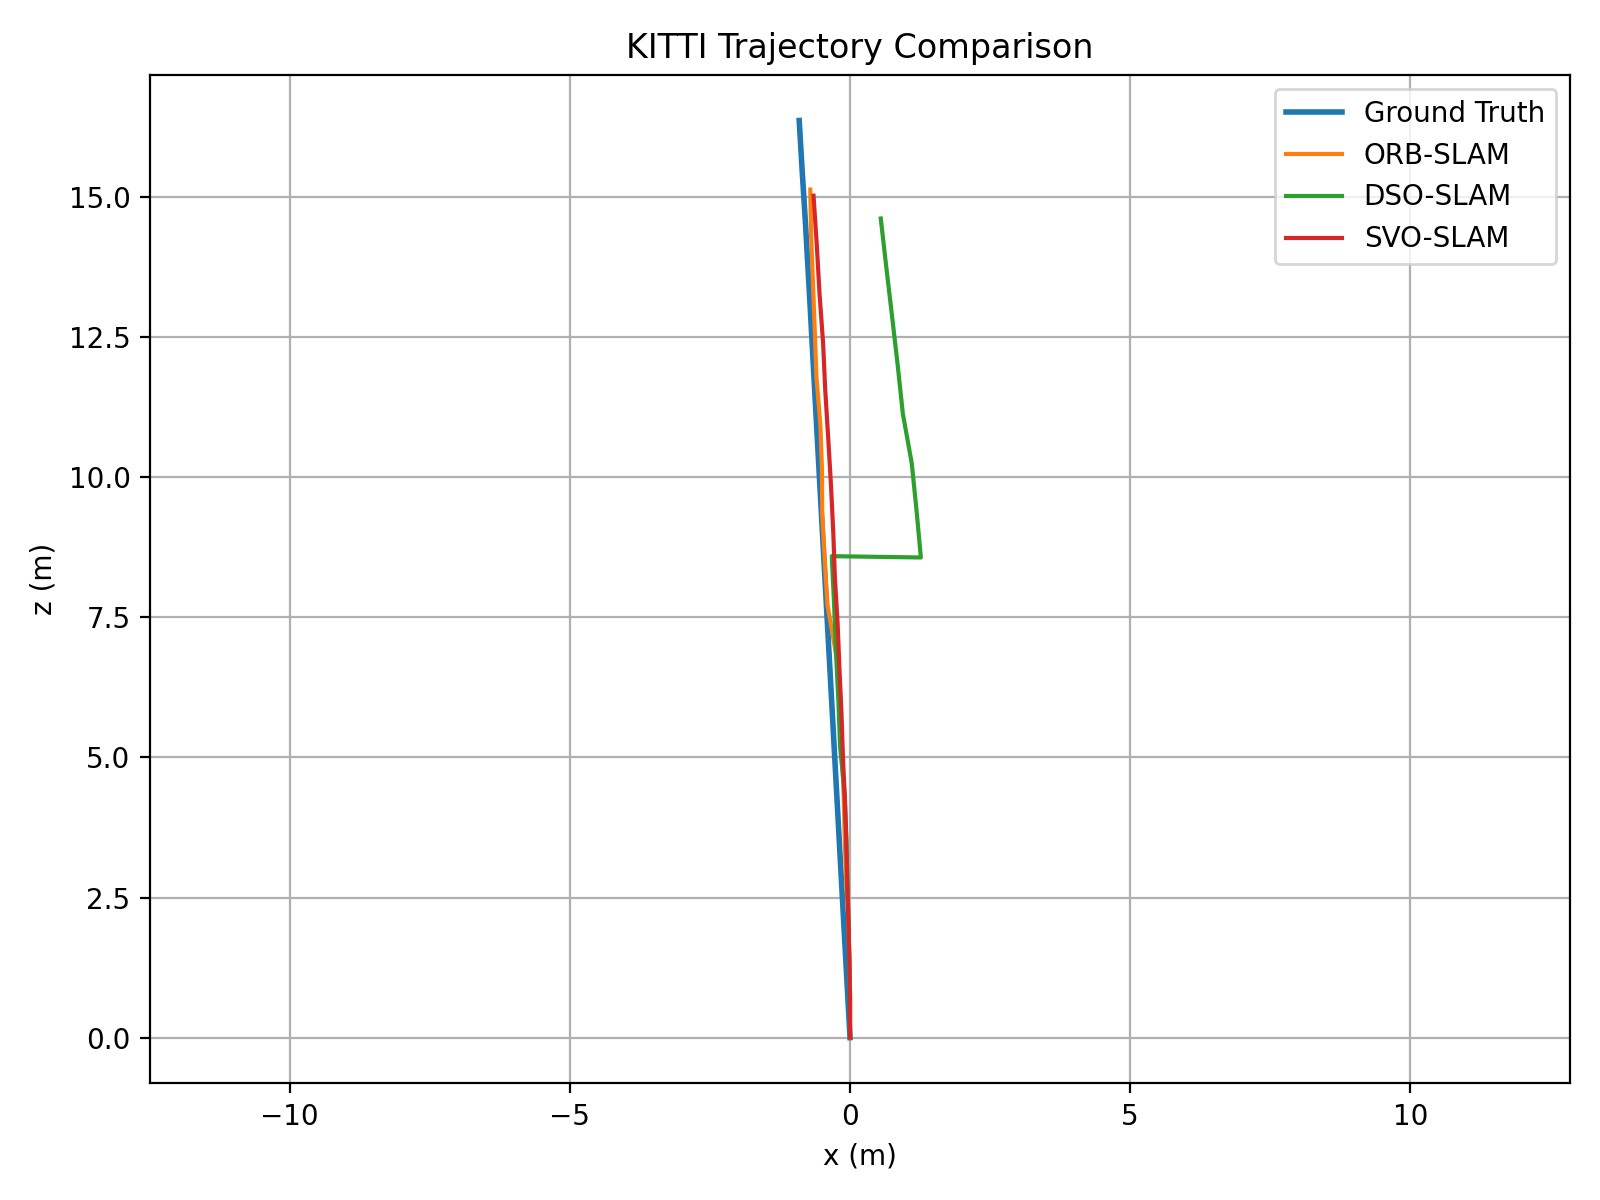
\includegraphics[width=0.76\textwidth]{sanity20_trajectory_seq00.png}
  \caption{Trajectory comparison for the first 20 frames of KITTI sequence 00. This sanity run confirms end-to-end execution and aligned output lengths for the three methods.}
  \label{fig:sanity-traj}
\end{figure}

\subsection{Analysis and Threats to Validity}

The main result indicates that the ORB-style baseline is the most accurate and robust method in the final 100-frame experiment. Its use of sparse descriptors, stereo depth, PnP RANSAC, and keyframe-based local mapping provides a stable implementation-level pipeline. However, its runtime is high in this Python implementation. The gap between median runtime and p95 runtime suggests that some frames trigger expensive local tracking, mapping, or optimization operations.

The SVO-style baseline achieves accuracy close to ORB-style while being much faster. This supports the intended role of the semi-direct design: it avoids full descriptor matching during tracking by using patch or optical-flow alignment, but it still estimates pose through sparse 3D-2D geometry. In the final run, this produces a favorable accuracy-runtime trade-off.

The DSO-style result must be interpreted carefully. It does not show that direct methods are inherently worse than feature-based methods. Instead, it shows that the simplified Python DSO-style baseline is sensitive to photometric assumptions, initialization quality, residual outliers, and incomplete joint optimization. Full DSO is a mature direct sparse odometry system with calibrated photometric modeling, sliding-window optimization, marginalization, and point lifecycle management. The project implementation uses only a subset of these ideas.

The main threats to validity are as follows. First, the final main experiment covers only the first 100 frames of KITTI sequence 00, so it does not represent all driving scenes or long-term drift behavior. Second, the final runs record zero loop closures, so the evaluation is closer to VO or local SLAM than to full long-term SLAM. Third, backend maturity differs across the baselines, so the comparison is not a ranking of the original algorithm families. Fourth, runtime values are local measurements because hardware specifications were not separately logged. Fifth, the 300-frame and full-sequence evaluations were not included due to computational cost.

\section{Research Conclusions}

This project implements and compares three Python visual SLAM/VO research baselines on KITTI Odometry: \methodorb{}, \methoddso{}, and \methodsvo{}. In the final 100-frame experiment on KITTI sequence 00, the ORB-style baseline obtains the best ATE RMSE of 1.8984 m with zero tracking failures. The SVO-style baseline obtains 2.3916 m ATE RMSE with zero tracking failures and substantially lower runtime. The DSO-style baseline obtains 9.4367 m ATE RMSE with 9 tracking failures and 9 fallbacks.

The results show that frontend design, point selection, outlier control, motion gating, and backend maturity jointly determine the behavior of a SLAM baseline. Under the current implementation constraints, feature-based tracking is the most stable, the semi-direct approach provides the best speed-accuracy compromise, and the simplified direct sparse approach requires stronger photometric modeling and joint optimization to reduce drift. The DSO ablation demonstrates that grid-uniform selection and outlier culling can materially reduce drift, while motion gating alone is insufficient when the residual set is unstable.

The conclusions should be understood as evidence about these Python research baselines, not as claims about the full official ORB-SLAM2, DSO, or SVO systems. Future work should include a more complete sliding-window photometric backend, stronger photometric calibration, more mature relocalization and loop closure, evaluation on additional KITTI sequences, complete hardware logging, and comparison with official C++ systems and modern deep SLAM methods under clearly separated protocols.

\section{Personnel and Task Division}

\begin{table}[H]
\centering
\caption{Personnel and task division.}
\label{tab:division}
\begin{tabular}{ll}
\toprule
Personnel & Task division \\
\midrule
24376333 Huang Yibo & Algorithm implementation and paper writing \\
24376267 Wang Xihao & Algorithm execution and checking; reference preparation \\
24301017 Yang Xiaochu & Experimental data preparation \\
\bottomrule
\end{tabular}
\end{table}

\bibliographystyle{ieeetr}
\bibliography{references}

\end{document}
